\section{Einleitung}
In diesem Versuch wird der Adiabatenexponent $\kappa$ mit Hilfe zweier
Methoden bestimmt.

Essentiell sind hier die Poissonschen Gleichungen, welche Druck, Volumen
und Temperatur bei adiabatischen Zustandsänderungen verknüpfen. Die
Poissonschen Gleichungen lauten,

\[
T\cdot V^{\kappa-1}=const'
\]
\begin{equation}
p\cdot V^{\kappa}=const''\label{eq:Poisson}
\end{equation}
\[
\frac{T^{\kappa}}{p^{\kappa-1}}=const'''
\]


unter Verwendung dieser Gleichungen lassen sich geschlossene Formeln
für $\kappa$ herleiten.

$\kappa$ ist der Quotient der molaren Wärmekapazitäten $c_{m,p}$und
$c_{m,V}$.

$c_{m,p}$ist die Wärmekapazität bei konstantem Druck und $c_{m,V}$
die Wärmekapazität bei konstantem Volumen, für $\kappa$ folgt,
\begin{equation}
\kappa=\frac{c_{m,p}}{c_{m,V}}=\frac{f+2}{f} \label{eq:freiheitsgrade}
\end{equation}


$f$ ist die Zahl der Freiheitsgrade.

Die erste Methode ist die Bestimmung von $\kappa$ nach Rüchard-Flammersfeld.
In diesem Versuchsaufbau befindet sich ein Glasrohr. welches mit einem
Gummistopfen an einer großen Flasche befestigt ist. In die Flasche
wird konstant entweder Luft, Argon oder CO2 hineingepumpt. Das Glasrohr
hat auf etwa halber Höhe einen Schlitz durch den Gas entweichen kann,
das Glasrohr besitzt die Fläche A.

In diesem Rohr befindet sich ein Schwingkörper, der durch das zuströmende
Gas und dem Schlitz zu einer harmonischen Schwingung angeregt wird.

Die Kreifrequenz lässt sich herleiten zu,
\begin{equation}
\omega^{2}=+\frac{\kappa p_{0}A^{2}}{mV_{0}}\label{eq:Frequenz}
\end{equation}


mit Hilfe der Schwingungsdauer $T=\frac{2\pi}{\omega}$ folgt für
$\kappa$,
\begin{equation}
\kappa=\frac{4\pi^{2}mV_{0}}{p_{0}A^{2}T^{2}} = \frac{4\pi^{2}mV_{0}f^2}{p_{0}A^{2}}\label{eq:adiabatenexponent}
\end{equation}


$V_{0}$und $p_{0}$sind Volumen und Druck des Gases in der Gleichgewichtslage,
$m$ ist die Masse des Schwingkörpers.

Somit kann anhand der Schwingungsdauer des Schwingkörpers der Adiabatenexponent
bestimmt werden.

Die zweite Methode ist die Bestimmung von $\kappa$ nach Clément-Desormes.

Bei dieser Methode ist ein großes Glasgefäß mit Luftgefüllt und mit
einem Flüssigketsbarometer verbunden. Während der Belüftungshahn geschlossen
ist wird der Druck im Gefäß erhöht.

Durch richtiges Timing beim Umdrehen des Hahns kann der Expansionsprozess
als adiabatisch angesehen werden. Durch weitere thermodynamische Überlegungen
und Annahmen und unter der Verwendung der Poissonschen Gleichungen
folgt für den Adiabatenexponent,
\begin{equation}
\kappa=\frac{h_{1}}{h_{1}-h_{3}}\label{eq:adiabatenexponent2}
\end{equation}


$h_{1}$ist die Höhe des Flüssigkeitsbarometers nachdem der Druck
erhöht wurde und $h_{3}$ist die Höhe nachdem der Hahn umgedreht wurde.
Mit Hilfe dieser Formel lässt sich mit diesem Versuchsaufbau der Adiabatenexponent
bestimmen. Mit \eqref{eq:freiheitsgrade} folgt daraus
\begin{equation}
f = 2\frac{h_1 - h_3}{h_3}
\end{equation}
\newpage

\section{Versuchsteil}

\subsection{Bestimmung von $ \kappa $ nach Rüchardt-Flammersfeld}
\subsubsection{Durchführung}
\begin{figure}[H]
\centering
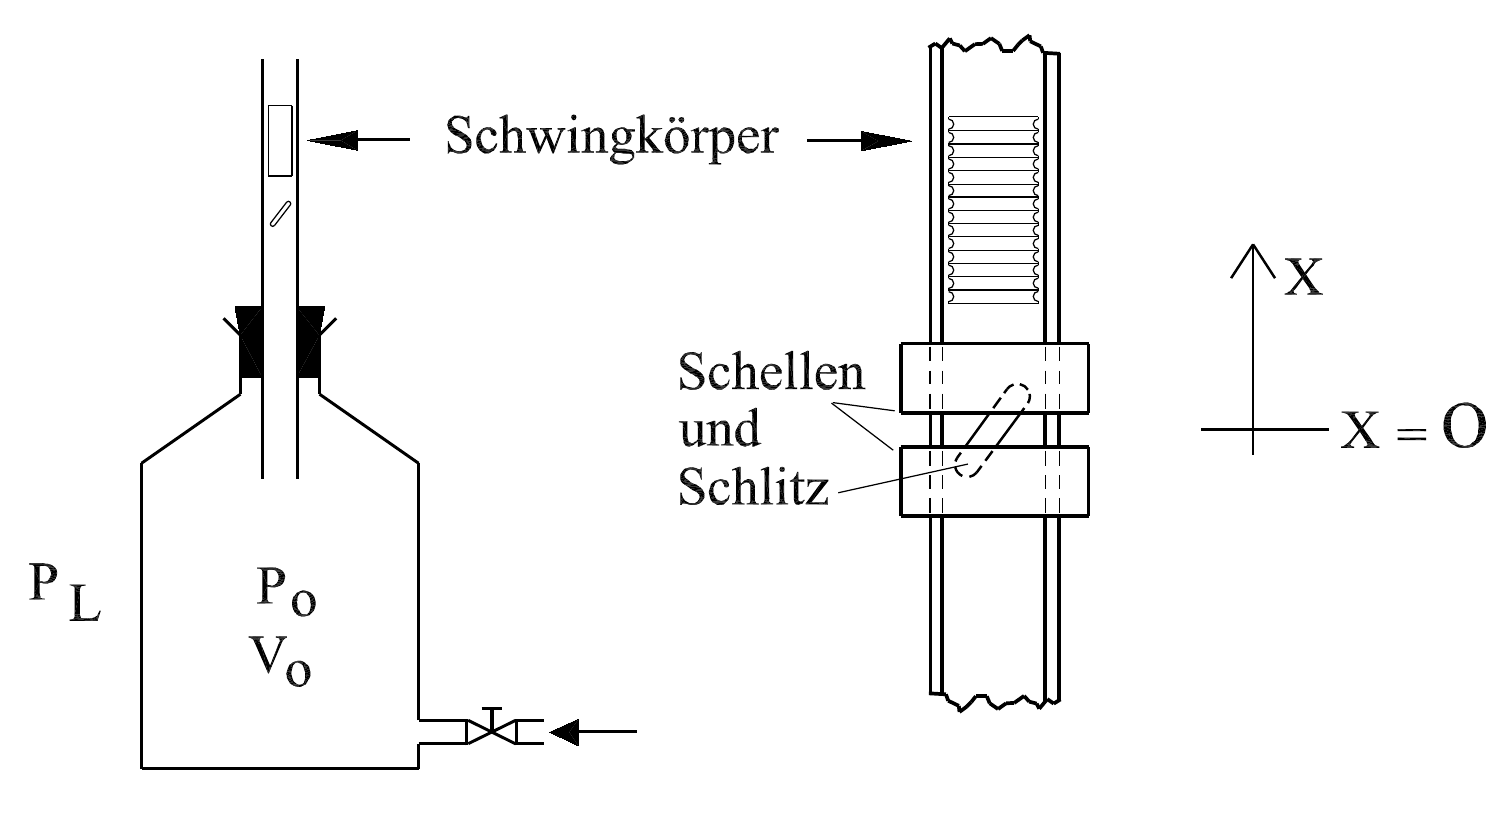
\includegraphics[width=0.7\linewidth]{./bilder/versuch1}
\caption{Versuchsaufbau nach Rüchardt-Flammersfeld (Quelle: \cite{anleitung2015})}
\label{fig:aufbau1}
\end{figure}

\def\vFlasche{5000}

\subsubsection{Auswertung}
Wenn der Schellenabstand verschwindet lässt sich mit \eqref{eq:adiabatenexponent} der Adiabatenexponent $ \kappa $ aus der Masse des Schwingkörpers, Volumen des Komprimierten Gases und dem Druck im Gleichgewicht zusammen. Die Masse des Schwingkörpers kann direkt gewogen werden und beträgt bei uns $ m = \SI{7,19(1)}{\g} $. Das Volumen setzt sich additiv aus dem Volumen der Flasche $ V_F = \SI{\vFlasche}{\cubic\centi\metre} $ und dem Volumen des Rohres zusammen. Das Volumen des Rohres wird aus Radius $ r $ und Höhe $ h $ bis zu Schlitz berechnet. Das ergibt $ V_R = \pi r^2 h = \SI{94,9(16)}{\cubic\centi\meter} $. Das Gesamtvolumen beträgt somit $ V = \dots $. %todo: Nachtragen
Der Druck $ p_0 $ setzt sich zusammen aus dem Umgebungsdruck von $ p_L = \SI{1011.7(1)}{\hecto\pascal} $ und dem von der Masse ausgeübten Druck $ p_m = \frac{mg}{A} = \frac{mg}{\pi r^2} = \SI{352,9 +- 4.5}{\pascal} $. Somit ist $ p_0 = \SI{1015.43 +- .15}{hPa} $.\\
Um die Frequenz zu ermitteln wird mit einem \textit{Least-Squares-Fit} eine Ausgleichsgerade durch die Messwerte gelegt. An den Abbildungen \ref{fig:luft} bis \ref{fig:co2} lässt sich damit der für eine verschwindene Spaltbreite extrapolierte Wert grafisch Ablesen.\\
Die so ermittelten Frequenzen betragen $ f_\mathrm L = \SI{1.880(15)}{\per\second} $ für Luft, \newline $ f_\mathrm{Ar} = \SI{1.910(15)}{\per\second} $ für Argon und $ f_{\mathrm{CO}_2} =~??? $ für \ch{CO2}. Setzt man dies mit den anderen Werten in \eqref{eq:adiabatenexponent} ein, erhält man die Adiabatenexponenten \newline
\begin{tabular}{l@{$~=~$}S[table-figures-integer = 1, table-figures-decimal = 3, table-figures-uncertainty = 3, table-number-alignment=left]}
$ \kappa_\mathrm{Luft} $ &  \\
$ \kappa_\mathrm{Ar} $ & \\
$ \kappa_{\mathrm{CO}_2} $
\end{tabular}
\begin{figure}[H]
\centering
\begin{tikzpicture}
\begin{axis}[width = .9\textwidth, height=8cm,
				xmin = 0, xmax = 3.5,
				xlabel = {Breite Spaltöffnung $ b $ [\si{\milli\meter}]},
				ylabel = {Schwingfrequenz $ f $ [\si{\per\second}]}]
	
	\addplot+[no marks] {-0.00763313 * x + 1.87894717};
	
	\addplot+ [only marks,
		error bars/.cd, y explicit, x explicit, x dir = both, y dir = both] table[x=x,y=y, x error = xerr, y error = yerr] {
x	xerr	y	yerr
3.00	0.05	1.858670875	0.0131324806
2.50	0.05	1.8566176471	0.0137589501
2.00	0.05	1.8642533937	0.0135781554
1.50	0.05	1.8674806967	0.0134838419
1.00	0.05	1.8695014663	0.0137713996
0.50	0.05	1.8770110833	0.0134617572
	};
	
	\legend{$ {\num{-0.0076}\cdot b + \num{1.8789}} $, Messwerte};
\end{axis}
\end{tikzpicture}
\caption{$ b $-$ f $-Diagramm mit Luft}
\label{fig:luft}
\end{figure}

\begin{figure}[H]
\centering
\begin{tikzpicture}
\begin{axis}[width = .9\textwidth, height=8cm,
				xmin = 0, xmax = 3.5,
				xlabel = {Breite Spaltöffnung $ b $ [\si{\milli\meter}]},
				ylabel = {Schwingfrequenz $ f $ [\si{\per\second}]},
				legend pos = south east]
	
	\addplot+[no marks] {0.02560155 * x + 1.90122003};
	
	\addplot+ [only marks,
		error bars/.cd, y explicit, x explicit, x dir = both, y dir = both] table[x=x,y=y, x error = xerr, y error = yerr] {
x	xerr	y	yerr
0.5	0.05	1.901076716	0.0127601693
1	0.05	1.9361778415	0.0137399449
1.5	0.05	1.9498607242	0.014290247
2	0.05	1.958937653	0.014533844
2.5	0.05	1.9487750557	0.0142776958
3	0.05	1.9813084112	0.0145182333
	};
	
	\legend{$ {\num{0.0256}\cdot b + \num{1.9012}} $, Messwerte};
\end{axis}
\end{tikzpicture}
\caption{$ b $-$ f $-Diagramm mit Argon}
\label{fig:ar}
\end{figure}

\begin{figure}[H]
\centering
\begin{tikzpicture}
\begin{axis}[width = .9\textwidth, height=8cm,
				xmin = 0, xmax = 3.5,
				xlabel = {Breite Spaltöffnung $ b $ [\si{\milli\meter}]},
				ylabel = {Schwingfrequenz $ f $ [\si{\per\second}]}]
	
	\addplot+[no marks] {0.00759521 * x + 1.81033195};
	
	\addplot+ [only marks,
		error bars/.cd, y explicit, x explicit, x dir = both, y dir = both] table[x=x,y=y, x error = xerr, y error = yerr] {
x	xerr	y	yerr
3	0.05	1.8481608987	0.0135278291
2.5	0.05	1.8117854002	0.0129909056
2	0.05	1.8236016132	0.0129957176
1.5	0.05	1.8305084746	0.0125877388
1	0.05	1.8010435954	0.0123912563
.5	0.05	1.8266413924	0.0127833737
	};
	
	\legend{$ {\num{0.0076}\cdot b + \num{1.8104}} $, Messwerte};
\end{axis}
\end{tikzpicture}
\caption{$ b $-$ f $-Diagramm mit \ch{CO2}}
\label{fig:co2}
\end{figure}

\subsection{Bestimmung von $ \kappa $ nach Clément-Desormes}
\subsubsection{Durchführung}
Zunächst wird im Behälter ein Druck aufgebaut. Da die Temperatur im Behälter dabei ansteigt muss daraufhin gewartet werden, bis sich der vom Manometer angezeigte Wert nicht mehr ändert und die Luft im Behältnis somit wieder die Umgebungstemperatur angenommen hat.
Nun misst man den Manometer-Stand $ h_1 $ ab.
Daraufhin wird sichergestellt, dass der Drucklufthahn geschlossen ist und der Belüftungshahn kurz aufgedreht. Dabei muss beachtet werden, dass wenn der Hahn zu kurz offen ist, sich nicht der gesamte Druck abbauen kann. Wird dagegen der Hahn zu lange offen gelassen, kann nicht mehr von Adiabasie\footnote{Der Begriff kommt aus der Versuchsanleitung} ausgegangen werden.\\
Durch die nach Möglichkeit adiabatische Expansion kommt es im Behälter zur Abkühlung während Umgebungsdruck herrscht.
Bei der Erwärmung baut sich wieder ein Druck auf und man ließt am Manometer $ h_3 $ ab.
%todo: Durchführung
\begin{figure}[H]
\centering
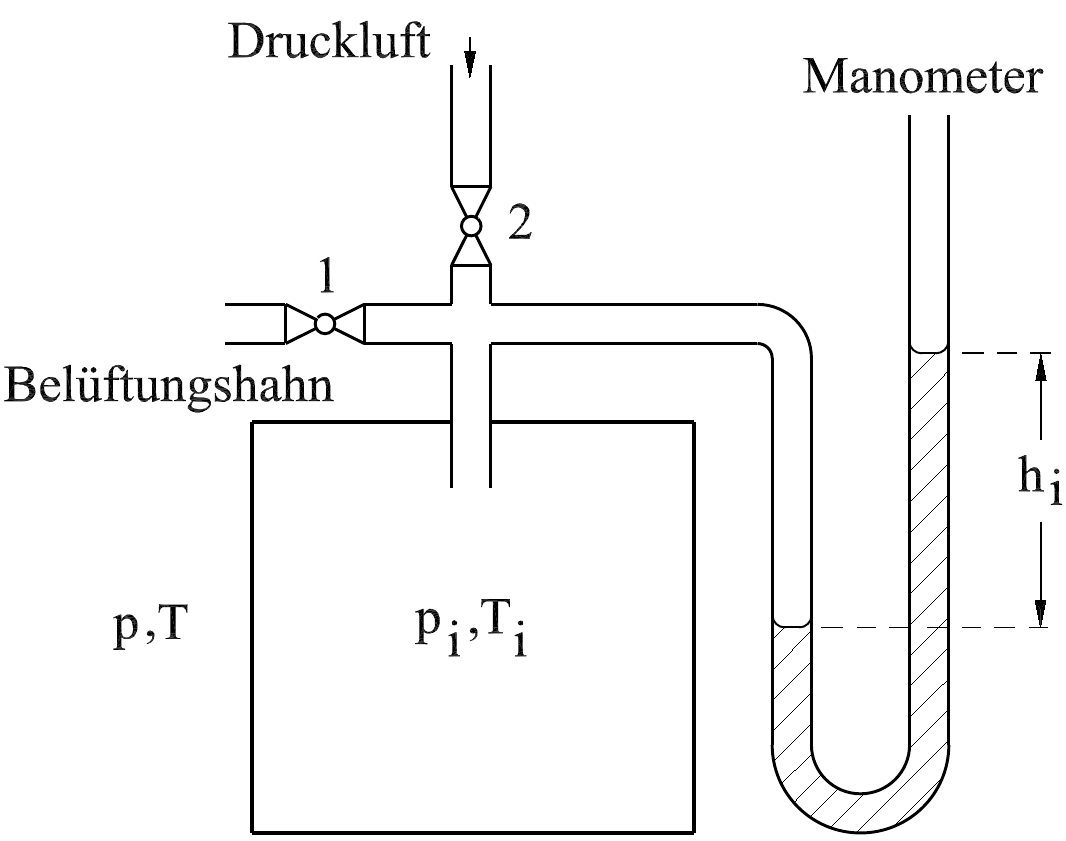
\includegraphics[width=0.7\linewidth]{./bilder/versuch2}
\caption{Aufbau nach Clément-Desormes (Quelle: \cite{anleitung2015})}
\label{fig:aufbau2}
\end{figure}

\subsubsection{Auswertung}
Aus $ h_1 $ und $ h_3 $ lassen sich mit \eqref{eq:adiabatenexponent2} und \eqref{eq:freiheitsgrade} Adiabatenexponent und Anzahl der Freiheitsgrade direkt berechnen. Die dazugehörigen Fehler erhält man aus \eqref{eq:err_k2} und \eqref{eq:err_f}. Daraus resultieren die Ergebnisse aus Tabelle \ref{tab:versuch2}. Im Mittel liegt die Zahl der Freiheitsgrade bei $ \bar f = \num{5.51(56)} $.
\begin{table}[H]
\centering
\sisetup{table-figures-integer = 1, table-figures-uncertainty = 1, table-figures-decimal = 1}
\begin{tabular}{
	S[ table-figures-integer = 2]
	S
	S[table-figures-decimal = 3,table-figures-uncertainty = 3]
	S[table-figures-uncertainty = 2, table-figures-decimal = 2]}
{$ h_1 [\si{\centi\meter}] $} & {$ h_3 [\si{\centi\meter}] $} & {$ \kappa $} & {$ f $} \\\hline\hline 
10,6 \pm 0,1 & 2,9 \pm 0,1 & 1,377 \pm 0,019 & 5,31 \pm 0,27 \\
10,6 \pm 0,1 & 2,7 \pm 0,1 & 1,342 \pm 0,018 & 5,85 \pm 0,31 \\
10,2 \pm 0,1 & 2,6 \pm 0,1 & 1,342 \pm 0,019 & 5,85 \pm 0,32 \\
13,5 \pm 0,1 & 3,6 \pm 0,1 & 1,364 \pm 0,015 & 5,50 \pm 0,22 \\
8,5 \pm 0,1 & 2,3 \pm 0,1 & 1,371 \pm 0,023 & 5,39 \pm 0,34 \\
8,2 \pm 0,1 & 2,3 \pm 0,1 & 1,390 \pm 0,025 & 5,13 \pm 0,33
\end{tabular}
\caption{Ergebnisse für $ \kappa $ und $ f $}
\label{tab:versuch2}
\end{table}

\newpage
\section{Diskussion} 

\subsection{Bestimmung von $ \kappa $ nach Clément-Desormes}
Da Stickstoff und Sauerstoff, die beiden Haupbestandteile der Luft, beides zweiatomige Gase sind, wären $ 5 $ Freiheitsgrade zu erwarten gewesen. Jedoch streuten unsere Messwerte zwischen \num{5.13} und \num{5.85}, bei einem Mittelwert von \num{5.51}. Somit läge nach unseren Ergebnissen nicht nur die erwartete Zahl im Konfidenzintervall, sondern auch \num{6} Freiheitsgrade.\\
